% Canonical pattern bodies adapted from pgflibrarypatterns.code.tex.
\documentclass[border=2pt]{standalone}
\usepackage{tikz}
\usetikzlibrary{patterns}

\begin{document}
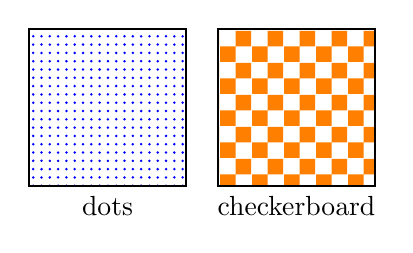
\begin{tikzpicture}
  \pgfdeclarepatternformonly{fixture dots}
    {\pgfqpoint{-1pt}{-1pt}}
    {\pgfqpoint{1pt}{1pt}}
    {\pgfqpoint{3pt}{3pt}}
    {
      \pgfpathcircle{\pgfpointorigin}{.5pt}
      \pgfusepath{fill}
    }
  \pgfdeclarepatternformonly{fixture checkerboard}
    {\pgfpointorigin}
    {\pgfqpoint{4mm}{4mm}}
    {\pgfqpoint{4mm}{4mm}}
    {
      \pgfpathrectangle{\pgfpointorigin}{\pgfqpoint{2mm}{2mm}}
      \pgfpathrectangle{\pgfqpoint{2mm}{2mm}}{\pgfqpoint{2mm}{2mm}}
      \pgfusepath{fill}
    }

  \fill[pattern=fixture dots,pattern color=blue] (0,0) rectangle (2,2);
  \fill[pattern=fixture checkerboard,pattern color=orange] (2.4,0) rectangle (4.4,2);
  \draw[thick] (0,0) rectangle (2,2);
  \draw[thick] (2.4,0) rectangle (4.4,2);
  \node[below] at (1,0) {dots};
  \node[below] at (3.4,0) {checkerboard};
\end{tikzpicture}
\end{document}
